\documentclass[11pt,a4paper]{article}

\usepackage[utf8]{inputenc}
\usepackage[T1]{fontenc}
\usepackage[margin=1in]{geometry}
\usepackage{tikz}
\usepackage{xcolor}
\usepackage{amsmath,amssymb}
\usepackage{booktabs}
\usepackage{hyperref}
\usepackage{enumitem}
\usepackage{fancyhdr}
\usepackage{titlesec}
\usepackage{float}

\usetikzlibrary{shapes.geometric, arrows.meta, positioning, calc, fit, backgrounds, patterns}

\definecolor{nemblue}{RGB}{91, 159, 207}
\definecolor{nemcyan}{RGB}{96, 192, 208}
\definecolor{nemdark}{RGB}{10, 22, 40}
\definecolor{yesgreen}{RGB}{96, 192, 128}
\definecolor{nored}{RGB}{192, 96, 112}
\definecolor{lobbyblue}{RGB}{112, 144, 192}
\definecolor{duelpurple}{RGB}{160, 112, 192}
\definecolor{gold}{RGB}{212, 168, 85}
\definecolor{mockgray}{RGB}{140, 140, 160}

\hypersetup{
    colorlinks=true,
    linkcolor=nemblue,
    urlcolor=nemcyan,
    citecolor=nemblue
}

\pagestyle{fancy}
\fancyhf{}
\fancyhead[L]{\textcolor{nemblue}{\textsc{Nemesis}}}
\fancyhead[R]{\textcolor{gray}{Hyperliquid London Community Hackathon 2026}}
\fancyfoot[C]{\thepage}
\renewcommand{\headrulewidth}{0.4pt}

\titleformat{\section}{\Large\bfseries\color{nemblue}}{\thesection}{1em}{}
\titleformat{\subsection}{\large\bfseries\color{nemcyan}}{\thesubsection}{1em}{}
\titleformat{\subsubsection}{\normalsize\bfseries\color{nemblue!70}}{\thesubsubsection}{1em}{}

\tikzset{
    box/.style={
        rectangle, rounded corners=4pt, minimum width=2.5cm, minimum height=1cm,
        draw=nemblue, fill=nemdark!80, text=white, font=\small\bfseries,
        align=center
    },
    greenbox/.style={box, draw=yesgreen, fill=yesgreen!20, text=nemdark},
    redbox/.style={box, draw=nored, fill=nored!20, text=nemdark},
    purplebox/.style={box, draw=duelpurple, fill=duelpurple!20, text=nemdark},
    bluebox/.style={box, draw=lobbyblue, fill=lobbyblue!20, text=nemdark},
    goldbox/.style={box, draw=gold, fill=gold!20, text=nemdark},
    mockbox/.style={box, draw=mockgray, fill=mockgray!15, text=nemdark, dashed},
    realbox/.style={box, draw=yesgreen, fill=yesgreen!10, text=nemdark, line width=1.5pt},
    saltbox/.style={box, draw=duelpurple, fill=duelpurple!15, text=nemdark, line width=1.5pt},
    arrow/.style={-{Stealth[length=3mm]}, thick, color=nemcyan},
    dasharrow/.style={-{Stealth[length=3mm]}, thick, dashed, color=gray},
    label/.style={font=\footnotesize, color=gray},
    user/.style={circle, minimum size=1cm, draw=nemblue, fill=nemblue!20, text=nemdark, font=\small\bfseries},
}

\begin{document}

\begin{titlepage}
    \centering
    \vspace*{2cm}

    {\Huge\bfseries\textcolor{nemblue}{NEMESIS}\par}
    \vspace{0.5cm}
    {\large\textit{\textcolor{nemcyan}{Every trader needs a Nemesis.}}\par}

    \vspace{2cm}

    {\Large\textcolor{gray}{Social Battle Trading Interface}\par}
    {\large\textcolor{gray}{on Hyperliquid}\par}

    \vspace{1.5cm}

    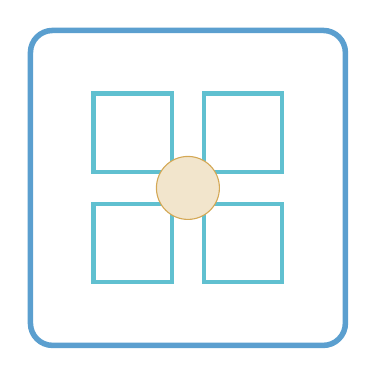
\begin{tikzpicture}
        \draw[nemblue, line width=2pt, rounded corners=8pt] (-2,-2) rectangle (2,2);
        \draw[nemcyan, line width=1.5pt] (-1.2,-1.2) rectangle (-0.2,-0.2);
        \draw[nemcyan, line width=1.5pt] (0.2,-1.2) rectangle (1.2,-0.2);
        \draw[nemcyan, line width=1.5pt] (-1.2,0.2) rectangle (-0.2,1.2);
        \draw[nemcyan, line width=1.5pt] (0.2,0.2) rectangle (1.2,1.2);
        \draw[gold, fill=gold!30] (0,0) circle (0.4);
    \end{tikzpicture}

    \vspace{2cm}

    {\large\textcolor{gray}{Hackathon Submission}\par}
    \vspace{0.3cm}
    {\normalsize\textcolor{gray}{LI.FI $\bullet$ Valantis $\bullet$ Pear Protocol $\bullet$ Salt $\bullet$ Insilico}\par}

    \vfill

    {\small\textcolor{gray}{January 2026}\par}
\end{titlepage}

\tableofcontents
\newpage

\section{Executive Summary}

Nemesis is a visual novel-inspired battle trading interface that transforms trading from a solitary activity into a social, competitive experience. Users can challenge rivals to direct counterparty arrangements, pool capital with friends, and participate in prediction markets on crypto price movements.

This document describes the hackathon submission targeting five sponsor tracks simultaneously, clearly distinguishing between what is implemented for the hackathon demonstration and what represents the prospective production system.

\begin{figure}[H]
\centering
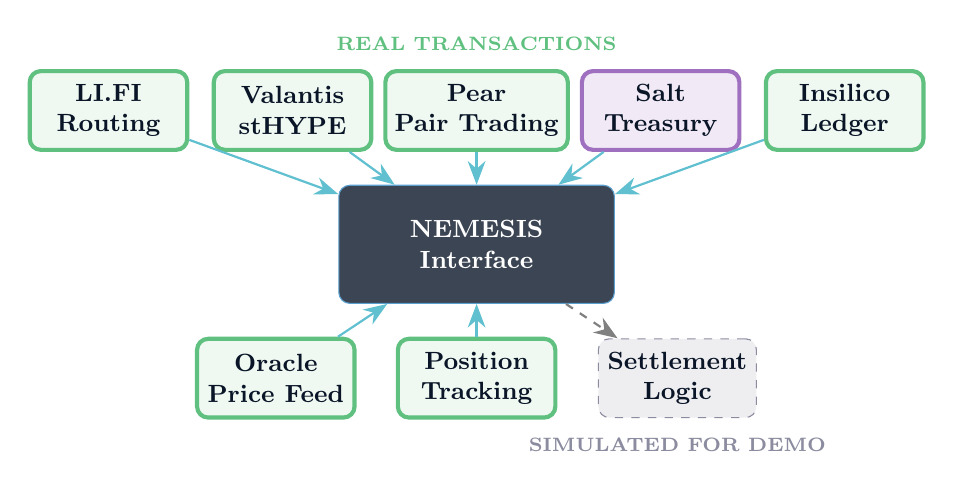
\begin{tikzpicture}[scale=0.85]
    \node[box, minimum width=3.5cm, minimum height=1.5cm] (nemesis) at (0,0) {NEMESIS\\Interface};

    \node[realbox, minimum width=2cm] (lifi) at (-5.5, 2) {LI.FI\\Routing};
    \node[realbox, minimum width=2cm] (valantis) at (-2.75, 2) {Valantis\\stHYPE};
    \node[realbox, minimum width=2cm] (pear) at (0, 2) {Pear\\Pair Trading};
    \node[saltbox, minimum width=2cm] (salt) at (2.75, 2) {Salt\\Treasury};
    \node[realbox, minimum width=2cm] (insilico) at (5.5, 2) {Insilico\\Ledger};

    \node[realbox, minimum width=2cm] (oracle) at (-3, -2) {Oracle\\Price Feed};
    \node[realbox, minimum width=2cm] (positions) at (0, -2) {Position\\Tracking};
    \node[mockbox, minimum width=2cm] (settlement) at (3, -2) {Settlement\\Logic};

    \draw[arrow] (lifi) -- (nemesis);
    \draw[arrow] (valantis) -- (nemesis);
    \draw[arrow] (pear) -- (nemesis);
    \draw[arrow] (salt) -- (nemesis);
    \draw[arrow] (insilico) -- (nemesis);
    \draw[arrow] (oracle) -- (nemesis);
    \draw[arrow] (positions) -- (nemesis);
    \draw[dasharrow] (nemesis) -- (settlement);

    \node[yesgreen, font=\scriptsize\bfseries] at (0, 3) {REAL TRANSACTIONS};
    \node[mockgray, font=\scriptsize\bfseries] at (3, -3) {SIMULATED FOR DEMO};
\end{tikzpicture}
\caption{Architecture showing real integrations (solid) versus simulated systems (dashed)}
\end{figure}

\subsection{Hackathon Scope}

The hackathon submission demonstrates real API integrations with all five sponsors wrapped in a compelling user experience. The prediction market functionality serves as the narrative context for these integrations.

\begin{table}[H]
\centering
\begin{tabular}{lcc}
\toprule
\textbf{Component} & \textbf{Hackathon Status} & \textbf{Transaction Type} \\
\midrule
Wallet Connection & Implemented & Real \\
LI.FI Cross-Chain Routing & Implemented & Real \\
Valantis stHYPE Deposit & Implemented & Real \\
Pear Pair Trading & Implemented & Real \\
Salt Organisation \& Robo Manager & Implemented & Real \\
Insilico Trade Ledger API & Implemented & Real \\
Oracle Price Feeds & Implemented & API Call \\
Trade History & Implemented & API Call \\
Position Tracking & Implemented & API Call \\
P\&L Calculations & Implemented & Computed \\
Leaderboard & Implemented & Computed \\
\midrule
Order Matching & Simulated & Local State \\
Settlement and Payouts & Not Implemented & Future Work \\
\bottomrule
\end{tabular}
\caption{Implementation status for hackathon submission}
\end{table}

\section{Product Vision}

\subsection{The Battle Trading Concept}

Traditional crypto trading is adversarial but impersonal. Nemesis makes the adversarial nature explicit and social through three mechanisms.

\subsubsection{Duels}

Direct one-on-one challenges between traders who disagree on a market outcome. User A believes ETH will exceed a price target; User B disagrees. They stake equal amounts in USDC, and the winner takes the combined stake minus platform fees.

\subsubsection{Trading Parties}

Friends pool capital and copy-trade together. When the party leader enters a position, members can automatically mirror the trade at a configurable ratio. Win together, lose together.

\subsubsection{Guilds}

Persistent groups with shared strategies implemented through Salt Organisations. Members create a Salt Organisation, set policies defining what the Nemesis Robo Manager can do on their behalf, and the bot executes strategies within those constraints automatically.

\begin{figure}[H]
\centering
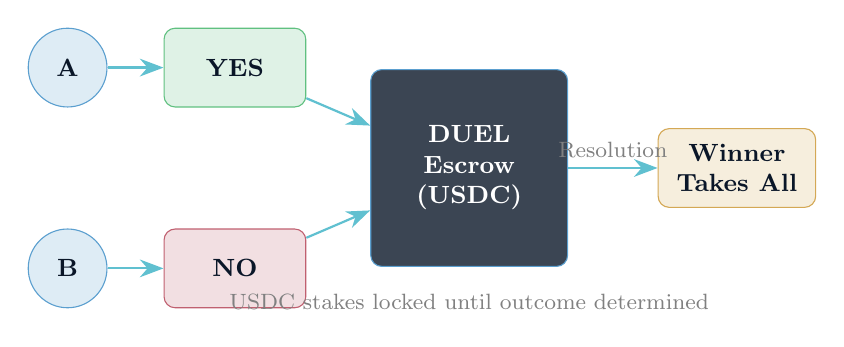
\begin{tikzpicture}[scale=0.85]
    \node[user] (alice) at (-4, 1.5) {A};
    \node[user] (bob) at (-4, -1.5) {B};

    \node[greenbox, minimum width=1.8cm] (yes) at (-1.5, 1.5) {YES};
    \node[redbox, minimum width=1.8cm] (no) at (-1.5, -1.5) {NO};

    \node[box, minimum width=2.5cm, minimum height=2.5cm] (duel) at (2, 0) {DUEL\\Escrow\\(USDC)};

    \node[goldbox, minimum width=2cm] (winner) at (6, 0) {Winner\\Takes All};

    \draw[arrow] (alice) -- (yes);
    \draw[arrow] (bob) -- (no);
    \draw[arrow] (yes) -- (duel);
    \draw[arrow] (no) -- (duel);
    \draw[arrow] (duel) -- node[above, label] {Resolution} (winner);

    \node[label] at (2, -2) {USDC stakes locked until outcome determined};
\end{tikzpicture}
\caption{Duel mechanics: direct counterparty arrangement with USDC escrow}
\end{figure}

\subsection{Visual Novel Interface}

The interface draws from Japanese visual novels with an AI avatar guiding users through the experience. This aesthetic choice serves the hackathon goal of attracting net new users by making trading approachable.

\begin{figure}[H]
\centering
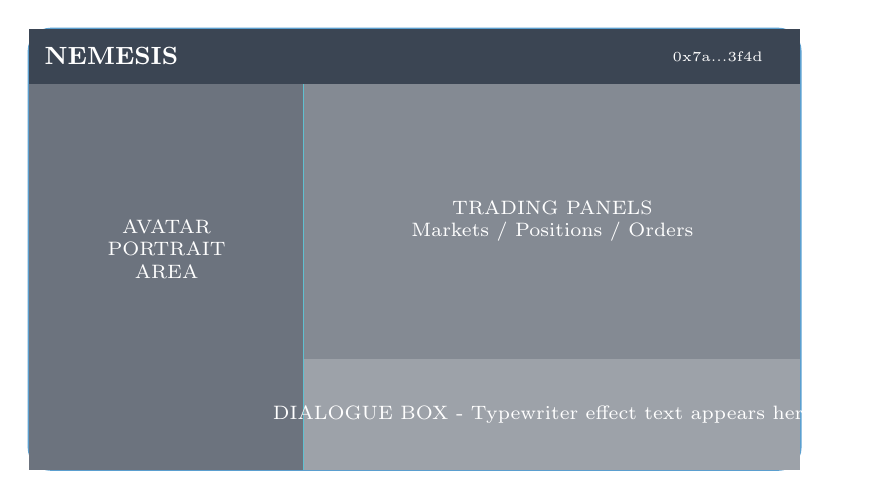
\begin{tikzpicture}[scale=0.7]
    \draw[nemblue, thick, rounded corners=8pt] (-7, -4) rectangle (7, 4);

    \fill[nemdark!80] (-7, 3) rectangle (7, 4);
    \node[white, font=\small\bfseries] at (-5.5, 3.5) {NEMESIS};
    \node[white, font=\tiny] at (5.5, 3.5) {0x7a...3f4d};

    \fill[nemdark!60] (-7, -4) rectangle (-2, 3);
    \node[white, font=\scriptsize, align=center] at (-4.5, 0) {AVATAR\\PORTRAIT\\AREA};

    \draw[nemcyan, thick] (-2, -4) -- (-2, 3);

    \fill[nemdark!40] (-2, -4) rectangle (7, -2);
    \node[white, font=\scriptsize] at (2.5, -3) {DIALOGUE BOX - Typewriter effect text appears here...};

    \fill[nemdark!50] (-2, -2) rectangle (7, 3);
    \node[white, font=\scriptsize, align=center] at (2.5, 0.5) {TRADING PANELS\\Markets / Positions / Orders};
\end{tikzpicture}
\caption{Interface layout: visual novel with trading panels}
\end{figure}

\section{Track Integrations}

\subsection{Track 1: LI.FI --- Cross-Chain Onboarding}

\textbf{Prize Pool:} \$6,000

Users arrive on any chain with any token and can onboard to HyperEVM with a single transaction. The LI.FI SDK handles routing, swapping, and bridging.

\begin{itemize}[leftmargin=*]
    \item User connects wallet on Ethereum, Arbitrum, Base, or other supported chain
    \item LI.FI finds optimal route to HyperEVM
    \item Single transaction moves funds cross-chain
    \item User lands on HyperEVM with USDC ready to trade
\end{itemize}

\subsection{Track 2: Valantis --- Liquid Staking}

\textbf{Prize Pool:} \$2,000

Valantis provides stHYPE, a liquid staking token for HYPE. Protocol treasury stakes HYPE to earn yield while maintaining liquidity.

\begin{itemize}[leftmargin=*]
    \item Protocol treasury accumulates HYPE from fees
    \item HYPE staked to Valantis stHYPE contract
    \item Yield accrues to protocol treasury
    \item User escrow remains in USDC (no HYPE price exposure for users)
\end{itemize}

\subsection{Track 3: Pear Protocol --- Pair Trading}

\textbf{Prize Pool:} \$3,500

Pear provides non-custodial pair and basket trading on Hyperliquid. Users can execute simultaneous long/short positions with a single transaction.

\begin{itemize}[leftmargin=*]
    \item Execution API for pair and basket trades
    \item Single-click open/close of long and short legs
    \item Market, limit, and TWAP order types
    \item Take-profit and stop-loss on price ratios
\end{itemize}

\subsection{Track 4: Salt --- Treasury Coordination}

\textbf{Prize Pool:} \$1,000

Salt is a treasury coordination platform using decentralised multi-party computation (dMPC). It enables self-custodial automated execution through policy-controlled accounts.

\subsubsection{Core Concepts}

\textbf{Robo Guardians} are an organisation's automated co-signers that enforce policies. They are hosted on the organisation's own infrastructure (AWS) and hold a portion of key material for every account. Robo Guardians will only co-sign transactions that pass all policy checks.

\textbf{Robo Managers} are third-party bots, humans, or AI agents that can execute transactions on an organisation's behalf without taking custody of assets. The pitch is: \textit{``Hire a bot. Keep custody.''}

\textbf{Nemesis as Robo Manager:} The Nemesis platform itself functions as a Robo Manager. Users create a Salt Organisation, invite Nemesis as a Robo Manager, set policies defining constraints, and Nemesis executes prediction market strategies on their behalf 24/7.

\begin{figure}[H]
\centering
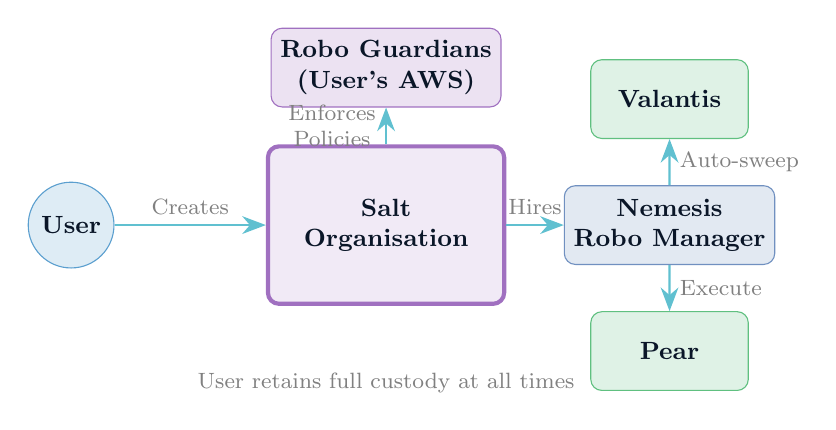
\begin{tikzpicture}[scale=0.8]
    \node[user] (user) at (-5, 0) {User};

    \node[saltbox, minimum width=3cm, minimum height=2cm] (org) at (0, 0) {Salt\\Organisation};

    \node[purplebox, minimum width=2.5cm] (guardians) at (0, 2.5) {Robo Guardians\\(User's AWS)};

    \node[bluebox, minimum width=2.5cm] (nemesis) at (4.5, 0) {Nemesis\\Robo Manager};

    \node[greenbox, minimum width=2cm] (valantis) at (4.5, 2) {Valantis};
    \node[greenbox, minimum width=2cm] (pear) at (4.5, -2) {Pear};

    \draw[arrow] (user) -- node[above, label] {Creates} (org);
    \draw[arrow] (org) -- node[left, label, align=center] {Enforces\\Policies} (guardians);
    \draw[arrow] (org) -- node[above, label] {Hires} (nemesis);
    \draw[arrow] (nemesis) -- node[right, label] {Auto-sweep} (valantis);
    \draw[arrow] (nemesis) -- node[right, label] {Execute} (pear);

    \node[label] at (0, -2.5) {User retains full custody at all times};
\end{tikzpicture}
\caption{Salt architecture: Nemesis as Robo Manager executing within policy constraints}
\end{figure}

\subsubsection{Policy Types}

Salt supports granular policy controls:

\begin{itemize}[leftmargin=*]
    \item \textbf{Allowed Recipients:} Whitelist of addresses the Robo Manager can interact with (e.g., only Pear and Valantis contracts)
    \item \textbf{Denied Recipients:} Blacklist of forbidden addresses
    \item \textbf{Transaction Limits:} Maximum amounts per transaction or time period
    \item \textbf{Nominated Approvers:} Require human approval for certain actions
\end{itemize}

\subsubsection{Implementation}

\begin{itemize}[leftmargin=*]
    \item \texttt{salt-sdk} npm package for TypeScript integration
    \item SIWE (Sign-In With Ethereum) authentication flow
    \item Organisation creation and member management
    \item Account setup with Robo Guardian coordination
    \item Policy definition and enforcement
    \item Transaction submission within policy constraints
    \item HyperEVM explicitly supported on mainnet and testnet
\end{itemize}

\subsection{Track 5: Insilico --- Trade Ledger API}

\textbf{Prize Pool:} \$5,000

Four API endpoints provide trade history, position tracking, P\&L calculations, and leaderboards. Data sourced from Hyperliquid Info API with abstraction layer for future data source swaps.

\begin{table}[H]
\centering
\begin{tabular}{llp{6cm}}
\toprule
\textbf{Endpoint} & \textbf{Method} & \textbf{Description} \\
\midrule
\texttt{/v1/trades} & GET & Trade history with filtering by user, coin, time range \\
\texttt{/v1/positions/history} & GET & Position timeline showing opens, modifications, closes \\
\texttt{/v1/pnl} & GET & Cumulative profit and loss calculations \\
\texttt{/v1/leaderboard} & GET & Ranked user performance aggregation \\
\bottomrule
\end{tabular}
\caption{Trade Ledger API endpoints}
\end{table}

\section{Business Model}

\subsection{Revenue Streams}

Nemesis generates revenue through two primary mechanisms:

\subsubsection{Duel Escrow Yield}

All prediction market escrow is denominated in USDC to provide defined risk without collateral volatility. While USDC is locked in escrow during active duels, it earns yield via lending protocols at approximately 3--8\% APY. Users receive their principal back; Nemesis retains the yield.

\begin{table}[H]
\centering
\begin{tabular}{lrr}
\toprule
\textbf{Metric} & \textbf{Conservative} & \textbf{Optimistic} \\
\midrule
TVL in Escrow & \$1,000,000 & \$10,000,000 \\
Average Lock Duration & 14 days & 14 days \\
Lending APY & 5\% & 8\% \\
Annual Yield Revenue & \$50,000 & \$800,000 \\
\bottomrule
\end{tabular}
\caption{Escrow yield revenue projections}
\end{table}

\subsubsection{Duel Fees}

A percentage of the winning pot or flat fee per duel creation. Fee structure to be determined based on market research and competitive analysis.

\subsubsection{Protocol Treasury}

Protocol treasury accumulates HYPE from fee conversion and stakes via Valantis for approximately 8\% APY. User escrow is never exposed to HYPE price risk---only protocol-owned funds are staked.

\subsection{Track Integrations as TVL Drivers}

The five track integrations are features that drive TVL, not direct revenue sources:

\begin{itemize}[leftmargin=*]
    \item \textbf{LI.FI:} Reduces friction $\rightarrow$ more users onboard $\rightarrow$ more escrow
    \item \textbf{Valantis:} Protocol treasury yield (not user escrow)
    \item \textbf{Pear:} Attracts traders $\rightarrow$ more duels $\rightarrow$ more escrow
    \item \textbf{Salt:} Guilds lock more capital $\rightarrow$ more escrow
    \item \textbf{Insilico:} Proves track records $\rightarrow$ attracts whales $\rightarrow$ more escrow
\end{itemize}

\section{Oracle Integration}

\subsection{Current: HyperCore Price Feeds}

\begin{itemize}[leftmargin=*]
    \item HyperCore Read precompile at \texttt{0x800} for gas-free price reads
    \item Real-time price updates for supported assets
    \item Market display reflects actual oracle prices
\end{itemize}

\subsection{Future: Settlement Oracle}

Settlement requires determining the asset price at market expiry to identify winners. This logic is not implemented for the hackathon but the oracle infrastructure is in place.

\begin{itemize}[leftmargin=*]
    \item Time-weighted average price (TWAP) to prevent manipulation
    \item Snapshot at market expiry timestamp
    \item Fallback oracles (Pyth, Chainlink) for redundancy
\end{itemize}

\section{Simulated Systems}

The following systems are simulated for the hackathon demonstration. They represent future development work required for a production prediction market.

\subsection{Order Matching}

Orders fill instantly without a matching engine.

\begin{itemize}[leftmargin=*]
    \item No order book implementation
    \item No counterparty matching
    \item Instant fill simulation for demonstration
\end{itemize}

\subsection{Settlement}

Market resolution and payout distribution are not implemented.

\begin{itemize}[leftmargin=*]
    \item No winner determination logic
    \item No fund distribution mechanism
    \item No escrow release automation
\end{itemize}

\section{Prospective Architecture}

This section describes the architecture required for a production prediction market. These components represent post-hackathon development.

\subsection{Smart Contract Requirements}

\begin{figure}[H]
\centering
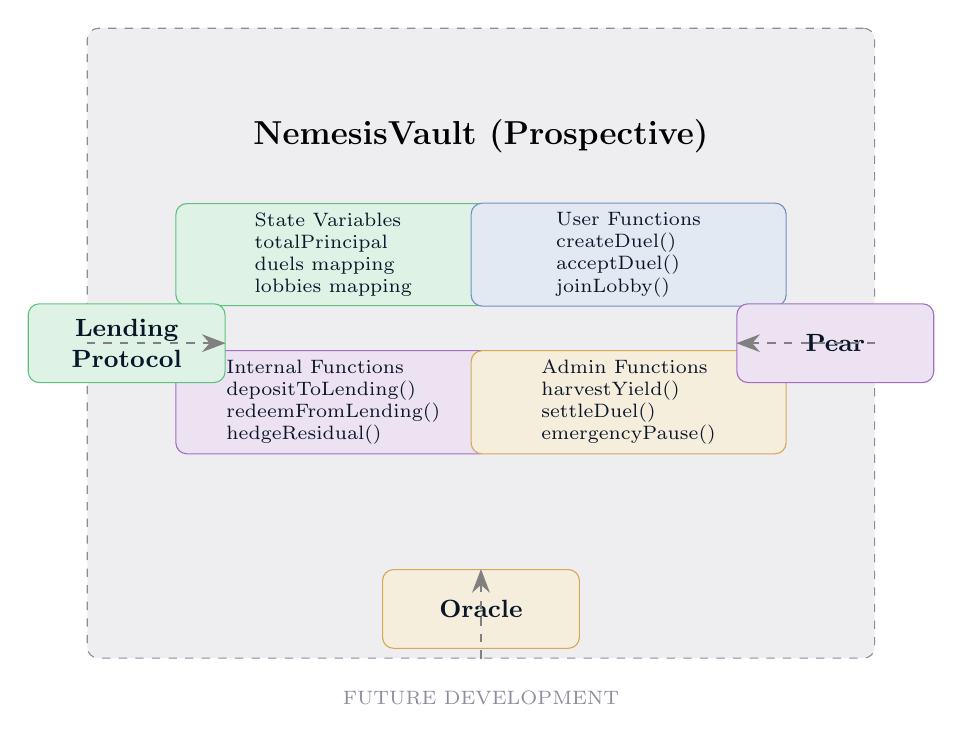
\begin{tikzpicture}[scale=0.75]
    \node[mockbox, minimum width=10cm, minimum height=8cm] (vault) at (0, 0) {};
    \node at (0, 3.5) {\textbf{\large NemesisVault (Prospective)}};

    \node[greenbox, minimum width=4cm, align=left, font=\scriptsize] at (-2.5, 1.5) {
        State Variables\\
        totalPrincipal\\
        duels mapping\\
        lobbies mapping
    };

    \node[bluebox, minimum width=4cm, align=left, font=\scriptsize] at (2.5, 1.5) {
        User Functions\\
        createDuel()\\
        acceptDuel()\\
        joinLobby()
    };

    \node[purplebox, minimum width=4cm, align=left, font=\scriptsize] at (-2.5, -1) {
        Internal Functions\\
        depositToLending()\\
        redeemFromLending()\\
        hedgeResidual()
    };

    \node[goldbox, minimum width=4cm, align=left, font=\scriptsize] at (2.5, -1) {
        Admin Functions\\
        harvestYield()\\
        settleDuel()\\
        emergencyPause()
    };

    \node[greenbox] (lending) at (-6, 0) {Lending\\Protocol};
    \node[purplebox] (pear) at (6, 0) {Pear};
    \node[goldbox] (oracle) at (0, -4.5) {Oracle};

    \draw[dasharrow] (vault) -- (lending);
    \draw[dasharrow] (vault) -- (pear);
    \draw[dasharrow] (vault) -- (oracle);

    \node[mockgray, font=\scriptsize] at (0, -6) {FUTURE DEVELOPMENT};
\end{tikzpicture}
\caption{Prospective smart contract architecture}
\end{figure}

\subsection{Internal Matching Engine}

A production system would match opposing bets internally before external hedging.

\begin{figure}[H]
\centering
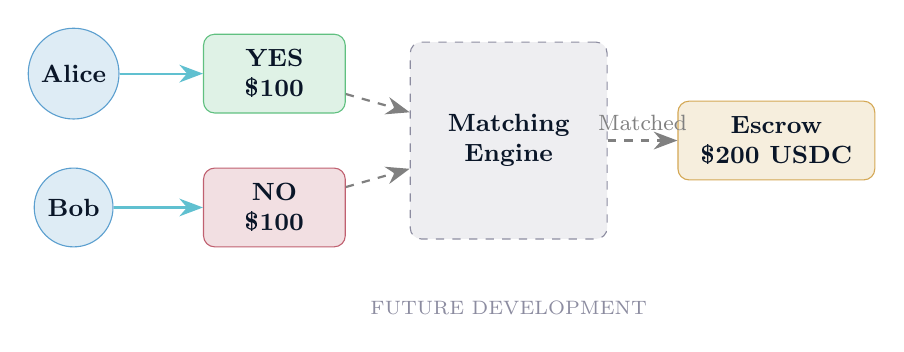
\begin{tikzpicture}[scale=0.85]
    \node[user] (alice) at (-4, 1) {Alice};
    \node[user] (bob) at (-4, -1) {Bob};

    \node[greenbox, minimum width=1.8cm] (yes) at (-1, 1) {YES\\\$100};
    \node[redbox, minimum width=1.8cm] (no) at (-1, -1) {NO\\\$100};

    \node[mockbox, minimum width=2.5cm, minimum height=2.5cm] (engine) at (2.5, 0) {Matching\\Engine};

    \node[goldbox, minimum width=2.5cm] (escrow) at (6.5, 0) {Escrow\\\$200 USDC};

    \draw[arrow] (alice) -- (yes);
    \draw[arrow] (bob) -- (no);
    \draw[dasharrow] (yes) -- (engine);
    \draw[dasharrow] (no) -- (engine);
    \draw[dasharrow] (engine) -- node[above, label] {Matched} (escrow);

    \node[mockgray, font=\scriptsize] at (2.5, -2.5) {FUTURE DEVELOPMENT};
\end{tikzpicture}
\caption{Prospective internal matching eliminates market exposure}
\end{figure}

\section{Development Roadmap}

\begin{table}[H]
\centering
\begin{tabular}{clp{6.5cm}}
\toprule
\textbf{Phase} & \textbf{Milestone} & \textbf{Deliverables} \\
\midrule
0 & Hackathon & Frontend, five track API integrations, oracle price feeds, trade ledger API \\
1 & Post-Hackathon & Smart contracts for escrow and matching, settlement logic \\
2 & Beta & Real order matching, settlement automation, audit \\
3 & Launch & Production deployment, liquidity bootstrapping \\
\bottomrule
\end{tabular}
\caption{Development roadmap from hackathon to production}
\end{table}

\subsection{Business Blockers}

The following must be addressed before launching as a production service:

\begin{table}[H]
\centering
\begin{tabular}{lp{7cm}}
\toprule
\textbf{Blocker} & \textbf{Description} \\
\midrule
Smart Contracts & Escrow, matching, and settlement logic \\
Settlement Logic & Winner determination and payout distribution \\
Liquidity & Counterparties for unmatched positions \\
Legal Structure & Prediction markets face regulatory requirements \\
Backend Infrastructure & Data serving at scale \\
\bottomrule
\end{tabular}
\caption{Requirements for production launch}
\end{table}

\section{Technical Stack}

\begin{table}[H]
\centering
\begin{tabular}{ll}
\toprule
\textbf{Component} & \textbf{Technology} \\
\midrule
Runtime & Bun \\
Build System & Nix Flakes \\
DOM Updates & morphdom \\
Wallet Connection & viem + @wagmi/core \\
Mobile Wallets & WalletConnect v2 \\
Cross-Chain Routing & @lifi/sdk \\
Pair Trading & Pear Protocol API \\
Treasury Coordination & salt-sdk \\
Liquid Staking & Valantis stHYPE \\
Price Feeds & HyperCore Oracle \\
Trade Ledger & Hyperliquid Info API \\
\bottomrule
\end{tabular}
\caption{Technology stack}
\end{table}

\subsection{Chain Configuration}

\begin{table}[H]
\centering
\begin{tabular}{lll}
\toprule
\textbf{Network} & \textbf{Chain ID} & \textbf{RPC} \\
\midrule
HyperEVM Mainnet & 999 & https://rpc.hyperliquid.xyz/evm \\
HyperEVM Testnet & 998 & https://rpc.hyperliquid-testnet.xyz/evm \\
Arbitrum (Salt Orchestration) & 42161 & https://arb1.arbitrum.io/rpc \\
\bottomrule
\end{tabular}
\caption{Chain configuration}
\end{table}

\section{Conclusion}

Nemesis demonstrates how five hackathon track technologies can integrate into a single coherent product. The visual novel interface provides an approachable entry point for new users, while the battle trading mechanics create social and viral growth potential.

The hackathon submission delivers:

\begin{itemize}[leftmargin=*]
    \item Real LI.FI integration for cross-chain routing
    \item Real Valantis integration for liquid staking yield
    \item Real Pear integration for pair trading
    \item Real Salt integration for treasury coordination via Robo Managers
    \item Real Insilico integration for trade ledger API
    \item Real oracle integration for live price feeds
    \item Polished frontend with visual novel aesthetic
    \item Simulated prediction market demonstrating the concept
\end{itemize}

The prospective production system would add smart contracts for escrow and settlement, winner determination logic, and the infrastructure required for a fully functional prediction market.

\vspace{1cm}
\begin{center}
\textit{\large Every trader needs a Nemesis.}
\end{center}

\end{document}
